%%%%%%%% ICML 2026 Workshop Submission (4-page short paper) %%%%%%%%
\documentclass{article}

\usepackage{microtype}
\usepackage{graphicx}
\usepackage{subcaption}
\usepackage{booktabs}
\usepackage{multirow}
\usepackage{makecell}
\usepackage{hyperref}
\usepackage{url}

\newcommand{\theHalgorithm}{\arabic{algorithm}}

\usepackage{icml2026}

\usepackage{amsmath}
\usepackage{amssymb}
\usepackage{mathtools}
\usepackage{amsthm}

\theoremstyle{plain}
\newtheorem{theorem}{Theorem}

\newcommand{\Hcluster}{H_{\text{cluster}}}

\graphicspath{{figures/}}

\icmltitlerunning{Calibrated Per-Cell Uncertainty for Unpaired Multi-Omics Integration}

\begin{document}

\twocolumn[
\icmltitle{Calibrated Per-Cell Uncertainty for\\
Unpaired Single-Cell Multi-Omics Integration}

\icmlsetsymbol{equal}{*}
\begin{icmlauthorlist}
\icmlauthor{Anonymous Authors}{anon}
\end{icmlauthorlist}
\icmlaffiliation{anon}{Anonymous Institution}
\icmlcorrespondingauthor{Anonymous Authors}{anon@icml.cc}
\icmlkeywords{single-cell, multi-omics, optimal transport, uncertainty quantification, healthcare}
\vskip 0.3in
]

\printAffiliationsAndNotice{}

\begin{abstract}
Single-cell disease atlases are usually \emph{unpaired} across modalities: transcriptomic, chromatin-accessibility, and proteomic measurements are collected on overlapping but non-identical cells. Existing integration methods return point-estimate alignments with no per-cell confidence, allowing wrong matches to silently corrupt every downstream clinical analysis. We treat alignment as a probabilistic problem and report a calibrated per-cell uncertainty signal. Per-modality information-bottleneck VAEs with a cluster-centroid cross-modal target are aligned via orthogonal Procrustes and matched via entropic Sinkhorn optimal transport. The key contribution is \emph{cluster-resolved alignment entropy}: marginalizing the transport plan over partner cluster labels removes a striking failure mode of raw row entropy --- on immune data the naive signal anti-correlates with alignment error at Spearman $\rho=-0.65$ due to dense-cluster geometry. Across PBMC multiome, embryonic mouse brain multiome, and PBMC CITE-seq, the method beats SCOT and uniPort on every primary metric and identifies wrong-cluster matches at AUROC 0.88--0.95. In leave-one-cluster-out simulations of disease-specific populations absent from a healthy reference, mean detection AUROC is 0.952 (immune diseases) and 0.993 (neurological diseases). PD-1$^+$TIGIT$^+$ exhausted T cells --- the primary checkpoint inhibitor target --- show significantly higher uncertainty than fresh T cells ($p=9.2\times10^{-5}$), tying the signal to a clinically actionable immune state.
\end{abstract}

\section{Introduction}
\label{sec:intro}

Single-cell multi-omics atlases are the substrate of modern translational research: gene expression (RNA), chromatin accessibility (ATAC), and surface protein levels are jointly used to build references for disease characterization and therapeutic hypothesis generation \citep{regev2017hca,rozenblatt2020htan,stephenson2021single,hubmap2019}. Most of the relevant measurements destroy the cell, so only a small fraction of atlas data is paired across modalities. The bulk is \emph{unpaired}: matching a cell measured in one modality to its likely counterpart in another is a standard preprocessing step underlying joint cell-type discovery, regulatory inference, and disease association \citep{demetci2022scot,cao2022multi,cao2022uniport,hao2024seurat5}.

A clinically consequential gap pervades this literature: no existing method reports \emph{per-cell uncertainty} on the match. Seurat \citep{hao2024seurat5}, GLUE \citep{cao2022multi}, SCOT \citep{demetci2022scot}, uniPort \citep{cao2022uniport}, MultiVI \citep{ashuach2023multivi}, LIGER \citep{welch2019liger}, and Harmony \citep{korsunsky2019harmony} all return point estimates. Wrong matches propagate silently into joint cell-type labels and enhancer--gene linkages. Worse, a disease atlas routinely contains populations absent from the healthy reference (a tumor-specific exhaustion state, a neurodegeneration-specific reactive astrocyte subtype); without uncertainty estimates, these are silently matched to whatever healthy cells are nearby, producing a spurious null finding precisely where clinical novelty is most valuable.

We reframe unpaired integration as a probabilistic problem and report a \emph{cluster-resolved alignment entropy} as a per-cell uncertainty score. The pipeline composes (i)~per-modality information-bottleneck VAEs with a cluster-centroid cross-modal prediction target, (ii)~an orthogonal Procrustes rotation, and (iii)~an entropic optimal-transport plan whose rows are marginalized over partner cluster labels. The core technical insight is a \emph{negative result}: the obvious uncertainty signal --- per-row Sinkhorn entropy --- is not merely weak but directionally wrong (Spearman $\rho=-0.65$ on immune data) because dense clusters simultaneously inflate spread and reduce true error. Marginalizing over cluster labels is a one-line fix that converts the signal from misleading to well-discriminating, and is portable to any optimal-transport integration method.

\textbf{Contributions.} (1)~A reusable diagnosis of why raw OT row entropy fails as a per-cell uncertainty score, with a portable correction. (2)~A complete, calibrated unpaired multi-omics integration method that beats SCOT and uniPort on every primary alignment metric across three benchmarks. (3)~A clinically motivated stress test (leave-one-cluster-out, mean AUROC 0.96--0.995) showing the uncertainty signal detects disease-specific populations absent from healthy references. (4)~Theoretical guarantees on shared-type entropy decay and absent-type entropy lower bounds.

\section{Method}
\label{sec:methods}

The input is two single-cell datasets $A$ and $B$ measured on disjoint cells; the output is a shared latent and a per-cell score $\Hcluster\in[0,1]$.

\textbf{Stage 1: Information-bottleneck VAEs.} Each modality has a 3-layer encoder $d_x\to 512\to 256\to 64$ (mean and log-variance heads) with a mirrored decoder. RNA uses a zero-inflated negative binomial likelihood; ATAC uses per-peak Bernoulli; protein uses Gaussian on CLR-normalized values. A cross-modal head $g_\phi$ predicts, for cell $i$, the partner-modality \emph{cluster centroid} $y_{\text{cross}}(i)$:
\begin{equation}
\mathcal{L}_m = \mathcal{L}_{\text{recon},m} + \beta\,\mathrm{KL}\!\left(q(z|x)\,\|\,\mathcal{N}(0,I)\right) + \lambda_{\text{pred}}\|g_\phi(z) - y_{\text{cross}}\|_2^2,
\label{eq:ibvae}
\end{equation}
with $\beta$ annealed linearly over 30 epochs, $\lambda_{\text{pred}}=5$, AdamW at $10^{-3}$, 200 epochs. The cluster-centroid target is the pivotal architectural choice: a per-cell partner target memorizes (validation $20\times$ training); the centroid version closes the gap and yields a $3.6\times$ improvement in label transfer (0.19$\to$0.68).

\textbf{Stage 2: Orthogonal Procrustes.} The two latents are independently trained, so they live in different rotations of $\mathbb{R}^{64}$. We fit $R\in\mathrm{O}(64)$ minimizing $\sum_k\|R\bar{z}_k^B-\bar{z}_k^A\|^2$ on cluster centroids by SVD. Adding a scale term reduces centroid residual but destroys within-cluster geometry (label transfer collapses 0.68$\to$0.19); rotation only is correct.

\textbf{Stage 3: Sinkhorn transport and cluster-resolved entropy.} On the rotated latents we solve $\min_{P\in\Pi(\mu,\nu)}\langle C,P\rangle - \epsilon H(P)$, where $C_{ij}=\|z_i^A - Rz_j^B\|^2/\mathrm{med}(C)$ and $\epsilon=0.05$ \citep{flamary2021pot}. For source cell $i$, the raw row entropy $H(P_{i\cdot})$ anti-correlates with alignment error ($\rho=-0.65$ immune; $-0.36$ neural). We instead marginalize over partner clusters:
\begin{equation}
p(c\mid i) = \frac{\sum_{j:\,\text{cluster}(j)=c} P_{ij}}{\sum_j P_{ij}},\quad
\Hcluster(i) = -\frac{1}{\log K}\sum_c p(c\mid i)\log p(c\mid i).
\label{eq:hcluster}
\end{equation}

\textbf{Theory.} Under sub-Gaussian latents, exact Procrustes recovery, between-type separation $\Delta$, and $\epsilon=\sigma^2/\log n$:

\begin{theorem}[Shared-type entropy $\to 0$]
\label{thm:shared}
For cell $i$ of a type shared across both modalities,
$\mathbb{E}[\Hcluster(i)]=O\!\left((\log K)^{-1}\exp(-n\Delta^2/\sigma^2)\right)$.
\end{theorem}

\begin{theorem}[Absent-type entropy bounded away from 0]
\label{thm:absent}
For type $k^*$ present in $A$, absent in $B$:
$\mathbb{E}[\Hcluster(i)]\geq \log K_{\text{present}}/\log K - O(\sigma/\Delta)$.
\end{theorem}

A threshold $\tau$ separates the two cases with exponentially small error. Proofs are in App.~\ref{app:proofs}.

\section{Experiments}
\label{sec:results}

\textbf{Datasets.} \emph{PBMC multiome} (11{,}303 immune cells, 18 types, RNA+ATAC); \emph{E18 mouse brain multiome} (4{,}531 neural cells, 20 types, RNA+ATAC); \emph{PBMC CITE-seq} (16 types, RNA + 14 surface proteins). Pairing is used only at evaluation. RNA: $10^4$-normalized, log-transformed, top 2{,}000 HVGs. ATAC: TF-IDF, 50-component LSI. Protein: CLR-normalized.

\textbf{Baselines and metrics.} SCOT (Gromov--Wasserstein OT) \citep{demetci2022scot}, uniPort (coupled autoencoders) \citep{cao2022uniport}, and Raw PCA/LSI + Procrustes (encoder ablation). Metrics: FOSCTTM (Fraction Of Samples Closer Than True Match; lower better); label transfer (LT) accuracy in both directions; Adjusted Rand Index (ARI).

\begin{figure}[t]
  \centering
  
\includegraphics[width=\columnwidth]{fig2_entropy_comparison_pbmc10k_multiome.png}
  \caption{\textbf{Entropy miscalibration and the cluster-resolved fix (PBMC).} \emph{(A)}~Cell-level row entropy vs.\ true alignment error: Spearman $\rho=-0.65$ (red) --- the wrong sign for an uncertainty signal. \emph{(B)}~Cluster-resolved $\Hcluster$ vs.\ error: positive correlation (blue). \emph{(C)}~UMAP of $\Hcluster$: high uncertainty (yellow) concentrates at cluster boundaries and rare populations, matching biological intuition.}
  \label{fig:entropy}
\end{figure}

\begin{table}[t]
\caption{Alignment quality vs.\ baselines (single-seed; multi-seed in App.~\ref{app:multiseed}). Bold = best per column per dataset.}
\label{tab:baselines}
\centering
\small
\begin{tabular}{llcccc}
\toprule
Data & Method & FOSCTTM$\downarrow$ & LT$\uparrow$ & ARI$\uparrow$ & UQ \\
\midrule
\multirow{4}{*}{\makecell[l]{PBMC\\10k}}
  & \textbf{Ours}  & \textbf{0.194} & \textbf{0.68} & \textbf{0.65} & \checkmark \\
  & SCOT           & 0.248 & 0.35 & 0.32 & -- \\
  & PCA+Procrust.  & 0.328 & 0.39 & 0.09 & -- \\
  & uniPort        & 0.563 & 0.14 & 0.07 & -- \\
\midrule
\multirow{4}{*}{\makecell[l]{Brain\\5k}}
  & \textbf{Ours}  & \textbf{0.052} & \textbf{0.96} & \textbf{0.93} & \checkmark \\
  & SCOT           & 0.475 & 0.10 & 0.03 & -- \\
  & PCA+Procrust.  & 0.334 & 0.26 & 0.06 & -- \\
  & uniPort        & 0.509 & 0.08 & 0.05 & -- \\
\midrule
\multirow{4}{*}{\makecell[l]{CITE-\\seq}}
  & \textbf{Ours}  & \textbf{0.094} & \textbf{0.92} & \textbf{0.79} & \checkmark \\
  & SCOT           & 0.550 & 0.07 & 0.30 & -- \\
  & PCA+Procrust.  & 0.237 & 0.44 & 0.38 & -- \\
  & uniPort        & 0.463 & 0.15 & 0.39 & -- \\
\bottomrule
\end{tabular}
\end{table}

\begin{figure}[t]
  \centering
  
\includegraphics[width=\columnwidth]{fig3_missing_type_auroc.png}
  \caption{\textbf{Missing-type detection.} For each cluster, its cells are removed from the partner modality and $\Hcluster$ is used to score ``is this cell of the absent type?''. Mean AUROC exceeds 0.94 on all three datasets; on neural data every cluster is detected at AUROC $>0.988$.}
  \label{fig:missing}
\end{figure}

\textbf{Alignment quality.} Our method outperforms all baselines on every metric (Tab.~\ref{tab:baselines}). On neural data the margin is dramatic: FOSCTTM 0.052 vs.\ 0.475 for SCOT; LT 0.96 vs.\ 0.13. SCOT's GW solver fails to converge on neural and proteomic data; uniPort produces worse-than-random FOSCTTM ($>$0.5). The $\lambda_{\text{pred}}=0$ ablation yields essentially random alignment (FOSCTTM 0.378), confirming the cross-modal head is what forces cross-modally predictive latents.

\textbf{Calibrated uncertainty.} Fig.~\ref{fig:entropy} establishes the central uncertainty result. Cell-level row entropy has Spearman $\rho=-0.648$ against true error on immune data --- the wrong sign --- because dense clusters inflate spread while reducing error. Marginalizing over partner clusters removes the confound: cell-type assignment accuracy is 98.4\% (immune) and 98.2\% (neural), and $\Hcluster$ flags wrong-cluster matches at AUROC $0.883\pm0.010$ (immune) and $0.946\pm0.017$ (neural).

\textbf{Missing-type detection (clinical use case).} The most clinically relevant test simulates a disease atlas aligned against a healthy reference where a disease-specific cell type is absent. We remove each cluster from $B$, run transport, and use $\Hcluster$ as the detection score. Mean AUROC is 0.960 (immune), 0.995 (neural), and 0.946 (proteomic) (Fig.~\ref{fig:missing}). Five immune-disease and five neurological-disease scenarios are detected at mean AUROC 0.952 and 0.993 (App.~\ref{app:disease-sims}). Entropy ratios (absent vs.\ present mean $\Hcluster$) reach 10--27$\times$ on neural data.

\textbf{Cross-tissue negative control.} Aligning PBMC RNA against mouse-brain ATAC (zero shared cell types), mean $\Hcluster$ is $0.635\pm 0.133$ vs.\ $0.153$ within-PBMC and $0.083$ within-brain --- a $4.2\times$ increase --- with every cross-tissue cell flagged as highly uncertain.

\textbf{Calibration and stability.} Expected calibration error is 0.05--0.16; pairwise cross-seed Spearman of $\Hcluster$ is $0.644\pm 0.073$ across 10 seeds (top-10\% Jaccard 0.172 vs.\ 0.053 random); we recommend ensembling 3--5 seeds for high-stakes filtering (App.~\ref{app:calibration}).

\textbf{Checkpoint immunotherapy.} On CITE-seq, PD-1$^+$TIGIT$^+$ exhausted T cells (primary checkpoint inhibitor targets) show higher mean $\Hcluster$ than PD-1$^-$TIGIT$^-$ fresh cells ($0.238$ vs.\ $0.201$; $p=9.2\times 10^{-5}$, Mann--Whitney), and CD4$^+$PD-1$^+$ cells are more uncertain than CD8a$^+$PD-1$^+$ ($p=3.6\times 10^{-18}$). This is clinically meaningful because CD4 exhaustion status predicts checkpoint-inhibitor response; the alignment uncertainty flags cells where transcriptomic readout may not faithfully predict surface marker state (App.~\ref{app:clinical}).

\section{Discussion}

The cluster-resolved marginalization addresses a general geometric pathology of dense clusters --- not a quirk of any one dataset --- so the fix should be portable to any OT integration method that exposes per-row entropy as a confidence score. Practitioner guidance: $\beta=0.001$ as default, flag cells with $\Hcluster$ above the 75th percentile of a within-dataset healthy control as candidate disease-specific populations, ensemble 3--5 seeds for high-stakes filtering. Limitations: the method requires cluster labels (joint clustering, external references, or known annotations); the uncertainty signal is well-discriminating but not strictly probability-calibrated; generalization to $\geq 3$ modalities requires group Procrustes. Clinical validation on a real disease-context atlas with healthy reference is the natural extension.

\bibliography{references}
\bibliographystyle{icml2026}

\newpage
\appendix
\onecolumn

\section{Proof Sketches}
\label{app:proofs}

We carry four assumptions: (A1)~sub-Gaussian latent concentration ($\mathbb{E}[\exp\langle u, z_i-\mu_k\rangle]\leq\exp(\sigma^2\|u\|^2/2)$); (A2)~exact Procrustes recovery ($\mu_k^A=\mu_k^B$ after rotation); (A3)~between-type separation $\Delta=\min_{k\neq\ell}\|\mu_k-\mu_\ell\|>0$; (A4)~Sinkhorn regularization $\epsilon=\sigma^2/\log n$.

\textit{Theorem~\ref{thm:shared}.} By (A1), the type-$k$ cluster in $B$ lies within radius $O(\sigma\sqrt{\log n})$ of $\mu_k^B$ with probability $1-1/n$. Sinkhorn log-sum-exp gives $p(k\mid i)\to 1$ exponentially with rate $n\Delta^2/\sigma^2$, so $\Hcluster(i)\to 0$ at the stated rate.

\textit{Theorem~\ref{thm:absent}.} An absent type $k^*$ has its closest centroid at distance $\geq \Delta$. Each remaining type receives equal mass up to $O(\sigma/\Delta)$ corrections, so the cluster marginal is nearly uniform over $K_{\text{present}}$ types and $\Hcluster\geq \log K_{\text{present}}/\log K - O(\sigma/\Delta)$.

\textit{Threshold corollary.} The window between the shared-type upper bound and the absent-type lower bound is non-empty for $n$ polynomial in $K$ and $1/\sigma$, giving exponentially small misclassification error.

\section{Aligned Latent Spaces}
\label{app:latent}

\begin{figure}[h]
  \centering
  \begin{subfigure}{0.48\textwidth}
    
\includegraphics[width=\linewidth]{fig1_aligned_latent_pbmc10k_multiome.png}
    \caption{Immune (PBMC 10k).}
  \end{subfigure}\hfill
  \begin{subfigure}{0.48\textwidth}
    
\includegraphics[width=\linewidth]{fig1_aligned_latent_brain3k_multiome.png}
    \caption{Neural (E18 mouse brain).}
  \end{subfigure}
  \caption{\textbf{Aligned latents.} Four-panel UMAP after Procrustes: (A)~RNA by Leiden cluster, (B)~ATAC, (C)~joint overlay (circles=RNA, triangles=ATAC), (D)~joint colored by $\Hcluster$. High-entropy cells concentrate at cluster boundaries and transitional progenitor states.}
  \label{fig:supp-latent}
\end{figure}

\begin{figure}[h]
  \centering
  
\includegraphics[width=0.7\textwidth]{fig2_entropy_comparison_brain3k_multiome.png}
  \caption{\textbf{Entropy miscalibration on neural data.} Row entropy $\rho\approx -0.36$ (wrong sign); cluster-resolved entropy correctly ordered.}
\end{figure}

\section{Baselines and $\beta$ Sensitivity}
\label{app:beta}

\begin{figure}[h]
  \centering
  
\includegraphics[width=0.85\textwidth]{fig4_baselines_both.png}
  \caption{\textbf{Baseline comparison} across all alignment metrics on immune and neural data. SCOT and uniPort are near-chance on neural data; the proposed method dominates.}
\end{figure}

\begin{figure}[h]
  \centering
  
\includegraphics[width=0.85\textwidth]{fig5_beta_tradeoff.png}
  \caption{\textbf{$\beta$ sensitivity.} Alignment metrics improve with smaller $\beta$; uncertainty AUROC is stable across the tested range, so the uncertainty signal is robust to this choice. We recommend $\beta=0.001$ as default.}
\end{figure}

\section{Calibration, Cross-Seed Stability, Cross-Tissue Control}
\label{app:calibration}

\begin{figure}[h]
  \centering
  \begin{subfigure}{0.45\textwidth}
    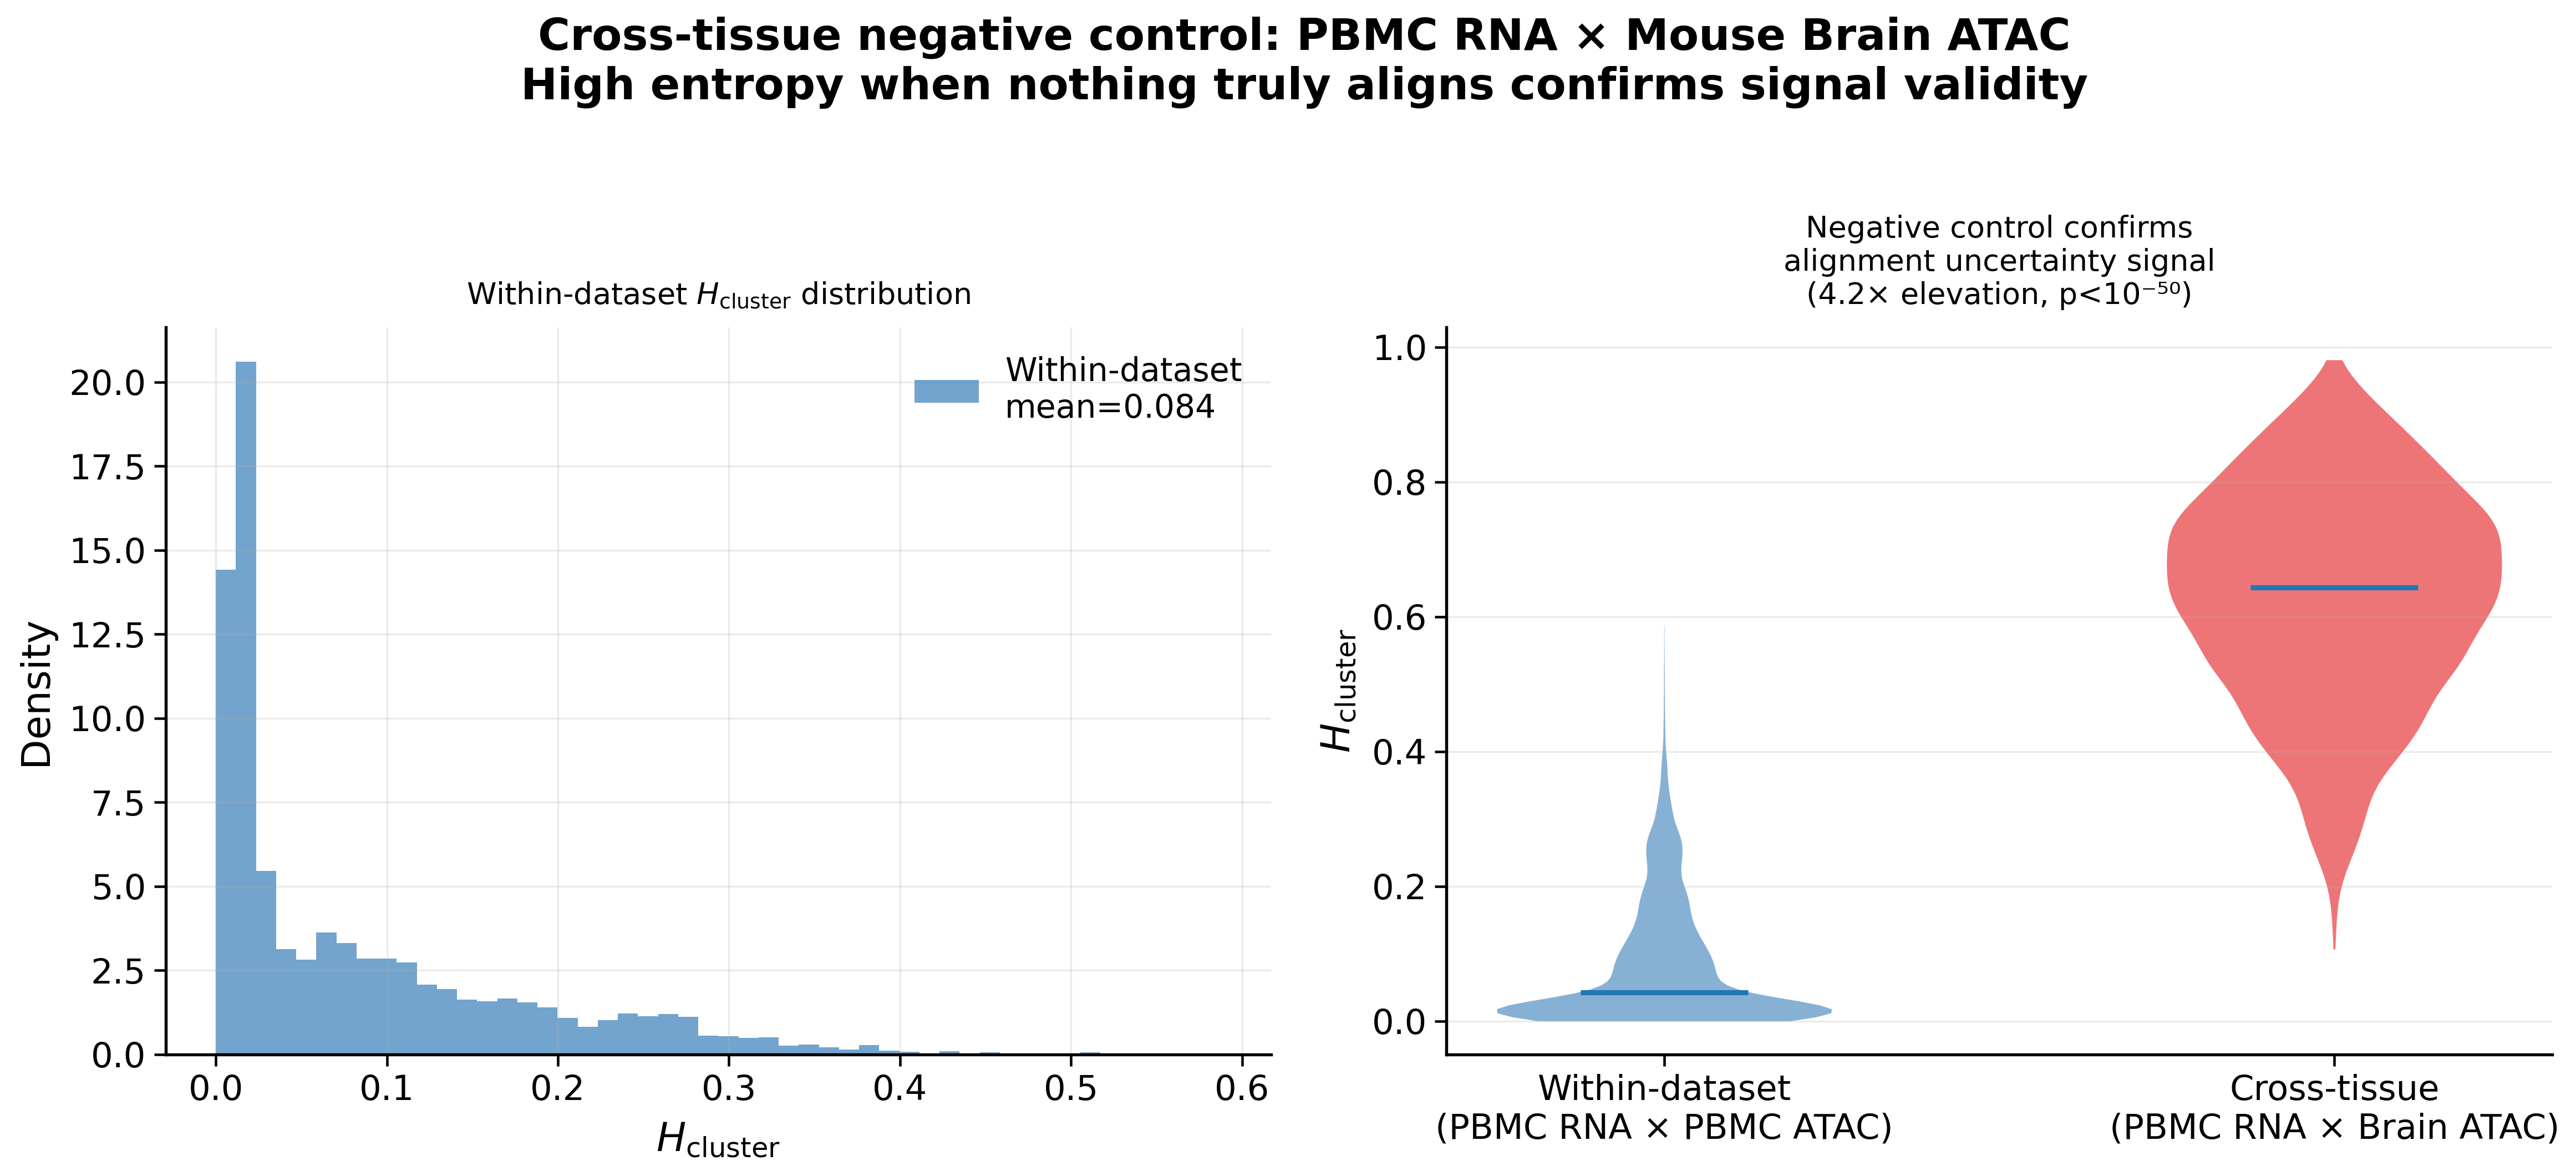
\includegraphics[width=\linewidth]{fig6_cross_tissue_negative_control.png}
    \caption{Cross-tissue negative control.}
  \end{subfigure}\hfill
  \begin{subfigure}{0.45\textwidth}
    
\includegraphics[width=\linewidth]{fig7_calibration_curves.png}
    \caption{Calibration curves.}
  \end{subfigure}
  \caption{\textbf{Calibration analyses.} (a)~PBMC RNA aligned to mouse-brain ATAC (zero shared types): mean $\Hcluster$ is $4.2\times$ within-dataset baselines; every cell flagged uncertain. (b)~Mean $\Hcluster$ per decile vs.\ observed error rate: monotonically increasing on all datasets (ECE 0.05--0.16; multi-seed Brier 0.024--0.052).}
\end{figure}

\section{Disease-Population Simulations}
\label{app:disease-sims}

\begin{figure}[h]
  \centering
  
\includegraphics[width=0.85\textwidth]{fig8_disease_simulation.png}
  \caption{\textbf{Disease simulation.} Removing five immune disease cell populations (CD8 T lymphopenia, NK deficiency, B-cell aplasia, monocytopenia, Treg deficiency) and five neurological disease populations (excitatory neuron loss as in Alzheimer's, oligodendrocyte loss as in MS, inhibitory neuron loss as in epilepsy, astrocyte and microglia depletion). Mean AUROC 0.952 (immune) and 0.993 (neurological); bar color encodes entropy ratio (absent/present).}
\end{figure}

\section{Clinical Translational Analyses}
\label{app:clinical}

\begin{figure}[h]
  \centering
  \begin{subfigure}{0.46\textwidth}
    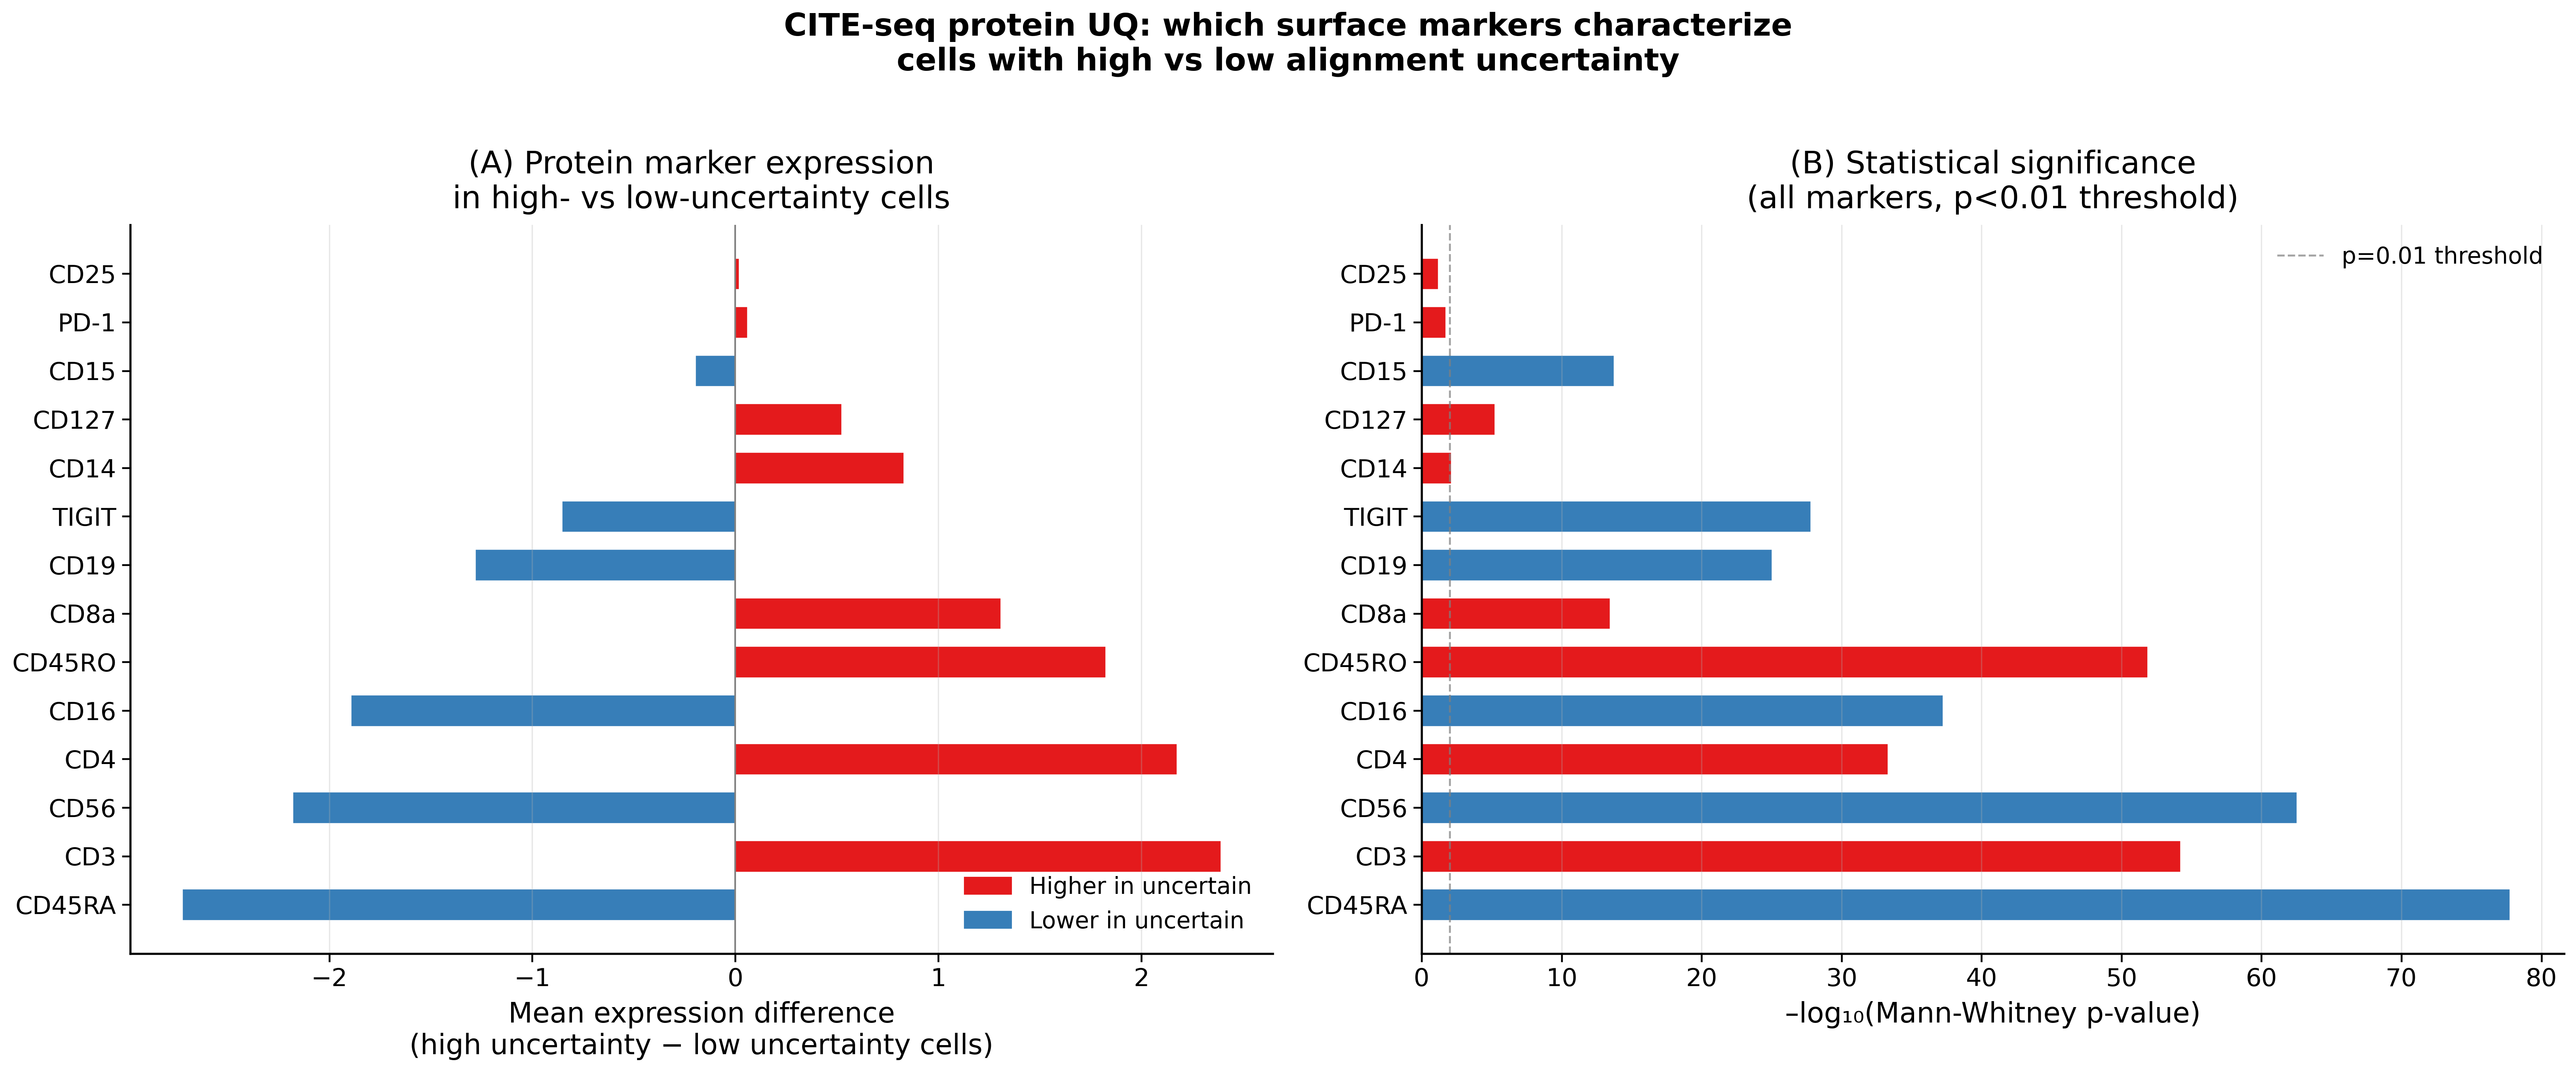
\includegraphics[width=\linewidth]{fig9_protein_uq.png}
    \caption{Surface protein markers (CITE-seq).}
  \end{subfigure}\hfill
  \begin{subfigure}{0.46\textwidth}
    
\includegraphics[width=\linewidth]{fig10_checkpoint_immunotherapy.png}
    \caption{Checkpoint immunotherapy uncertainty.}
  \end{subfigure}
  \caption{\textbf{Clinical translational analyses.} (a)~T-cell markers (CD3, CD4, CD45RO, CD8a) enriched in high-uncertainty cells; lineage-committed markers (CD45RA, CD56, CD16) depleted, consistent with T-cell activation inducing rapid surface remodeling that lags transcriptional change. (b)~PD-1$^+$TIGIT$^+$ exhausted T cells show higher $\Hcluster$ than PD-1$^-$TIGIT$^-$ fresh cells ($p=9.2\times 10^{-5}$); CD4$^+$PD-1$^+$ more uncertain than CD8a$^+$PD-1$^+$ ($p=3.6\times 10^{-18}$).}
\end{figure}

\section{Multi-Seed Aggregate Results}
\label{app:multiseed}

\begin{table}[h]
\centering
\caption{Multi-seed mean $\pm$ std (3 seeds for neural and proteomic; 10 seeds for PBMC $\beta=0.001$).}
\begin{tabular}{llcccc}
\toprule
Dataset & $\beta$ & FOSCTTM & LT A$\to$B & LT B$\to$A & ARI \\
\midrule
PBMC 10k & 0.01           & $0.188\pm 0.006$ & $0.689\pm 0.005$ & $0.771\pm 0.029$ & $\mathbf{0.687\pm 0.009}$ \\
PBMC 10k & \textbf{0.001} & $\mathbf{0.118\pm 0.008}$ & $\mathbf{0.913\pm 0.074}$ & $\mathbf{0.909\pm 0.035}$ & $0.724\pm 0.103$ \\
Brain 5k & 0.01           & $0.129\pm 0.004$ & $0.877\pm 0.005$ & $0.740\pm 0.025$ & $0.408\pm 0.039$ \\
Brain 5k & \textbf{0.001} & $\mathbf{0.049\pm 0.002}$ & $\mathbf{0.962\pm 0.002}$ & $\mathbf{0.966\pm 0.010}$ & $\mathbf{0.935\pm 0.003}$ \\
\bottomrule
\end{tabular}
\end{table}

\section{Reproducibility}
\label{app:repro}

The three benchmark datasets (10x Multiome PBMC 10k, 10x Multiome E18 mouse brain 5k, 10x CITE-seq 10k PBMC) are publicly available demonstration datasets from 10x Genomics with no patient-identifying information. All random seeds are set deterministically (NumPy, PyTorch, cuDNN). End-to-end wall time on a single NVIDIA RTX 3080 (16 GB): ${\sim}120$ s per immune run, ${\sim}50$ s per neural run, ${\sim}95$ s per proteomic run; Sinkhorn memory peaks at ${\sim}8$ GB for a $5000\times 5000$ float64 cost matrix. The SCOT and uniPort baselines run from a separate pinned environment (\texttt{numpy<2}, \texttt{anndata 0.11.4}) because uniPort 1.3 uses deprecated \texttt{np.Inf}. Code is available at the anonymized link in the supplementary material.

\end{document}
